%%%%%%%%%%%%%%%%%%%%%%%%%%%%%%%%%%%%%%%%%%%%%%%%%%%%%
%                                                   %
%     Penn State Colloquium Poster Template         %
%                                                   %
% Uses Penn State Colloquium class, with options:   %
%                                                   %
% Orientation:                                      %
%     portrait (default), landscape                 %
%                                                   %
% Paper size:                                       %
%     a4paper (default), a0paper, a1paper, a2paper, %
%     a3paper, a5paper, a6paper                     %
%%%%%%%%%%%%%%%%%%%%%%%%%%%%%%%%%%%%%%%%%%%%%%%%%%%%%
\documentclass{../psuposter}
\renewcommand{\templateimagepath}{../} 


%%%%%%%%%%%%%%%%%%%%%%%%%%%%%%%%%%%%%%%%%%%%%%%%%%%%%
%               Package Dependencies                %
%%%%%%%%%%%%%%%%%%%%%%%%%%%%%%%%%%%%%%%%%%%%%%%%%%%%%
\usepackage{natbib}
\usepackage{lipsum}                                % Dummy text
\usepackage[figwidth = 0.98\linewidth]{todonotes}  % Dummy image (and more!)
\usepackage[absolute, overlay]{textpos}            % Figure placement
\usepackage{braket}
\setlength{\TPHorizModule}{\paperwidth}
\setlength{\TPVertModule}{\paperheight}
\setcitestyle{numbers,square}


%%%%%%%%%%%%%%%%%%%%%%%%%%%%%%%%%%%%%%%%%%%%%%%%%%%%%
%                 AUTHOR AND TITLE                  %
%%%%%%%%%%%%%%%%%%%%%%%%%%%%%%%%%%%%%%%%%%%%%%%%%%%%%
\title{POEMMA \& EUSO-SPB to observe the Highest Energy Particles from Space}
\author{Angela Olinto}
\institute{The University of Chicago}


%%%%%%%%%%%%%%%%%%%%%%%%%%%%%%%%%%%%%%%%%%%%%%%%%%%%%
%                  BEGIN DOCUMENT                   %
%%%%%%%%%%%%%%%%%%%%%%%%%%%%%%%%%%%%%%%%%%%%%%%%%%%%%
\begin{document}
\begin{frame}
\begin{columns}[t, totalwidth=\textwidth]
\begin{column}{0.45\textwidth - 1cm}


%%%%%%%%%%%%%%%%%%%%%%%%%%%%%%%%%%%%%%%%%%%%%%%%%%%%%
%                 BLOCK: BIOGRAPHY                  %
%%%%%%%%%%%%%%%%%%%%%%%%%%%%%%%%%%%%%%%%%%%%%%%%%%%%%
    \begin{block}{Speaker Biographic Summary}
    	\begin{center}
    		
\includegraphics[width=0.6\textwidth]{images/portrait}
    	\end{center}
    	\href{https://president.uchicago.edu/directory/angela-olinto}{Dr. Angela Olinto}  is Dean of the Division of the Physical Sciences and the Albert A. Michelson Distinguished Service Professor in the Department of Astronomy and Astrophysics, the Kavli Institute for Cosmological Physics, and the Enrico Fermi Institute at the University of Chicago. 
%    	She previously served as Chair of the Department of Astronomy and Astrophysics from 2003 to 2006 and again from 2012 to 2017.
			Olinto is best known for her contributions to the study of the structure of neutron stars, primordial inflationary theory, cosmic magnetic fields, the nature of the dark matter, and the origin of the highest energy cosmic rays, gamma-rays, and neutrinos. She is the Principal Investigator of the POEMMA space mission and the EUSO on a super pressure balloon mission.
			Olinto received a B.S. in Physics from the Pontifícia Universidade Católica of Rio de Janeiro, Brazil in 1981, and Ph.D. in Physics from MIT in 1987. She is a fellow of the APS and the AAAS, was a trustee of the Aspen Center for Physics.
%			, and has served on many advisory committees for the National Academy of Sciences, Department of Energy, National Science Foundation, and the National Aeronautics and Space Administration. 
			She received the Chaire d’Excellence Award of the French Agence Nationale de Recherche in 2006, the Llewellyn John and Harriet Manchester Quantrell Award for Excellence in Undergraduate Teaching in 2011, and the Faculty Award for Excellence in Graduate Teaching in 2015 at the University of Chicago.
    \end{block}


%%%%%%%%%%%%%%%%%%%%%%%%%%%%%%%%%%%%%%%%%%%%%%%%%%%%%
%            BLOCK: RESEARCH INTERESTS              %
%%%%%%%%%%%%%%%%%%%%%%%%%%%%%%%%%%%%%%%%%%%%%%%%%%%%%
    \begin{block}{Research Interests}
        Olinto's interests are in theoretical astrophysics, particle and nuclear astrophysics, and cosmology. Her work has focused on the highest energy cosmic rays, indirect signatures of particle dark matter, cosmological effects of magnetic fields, natural inflation, and the internal structure of neutron stars. 
        \begin{center}
	    	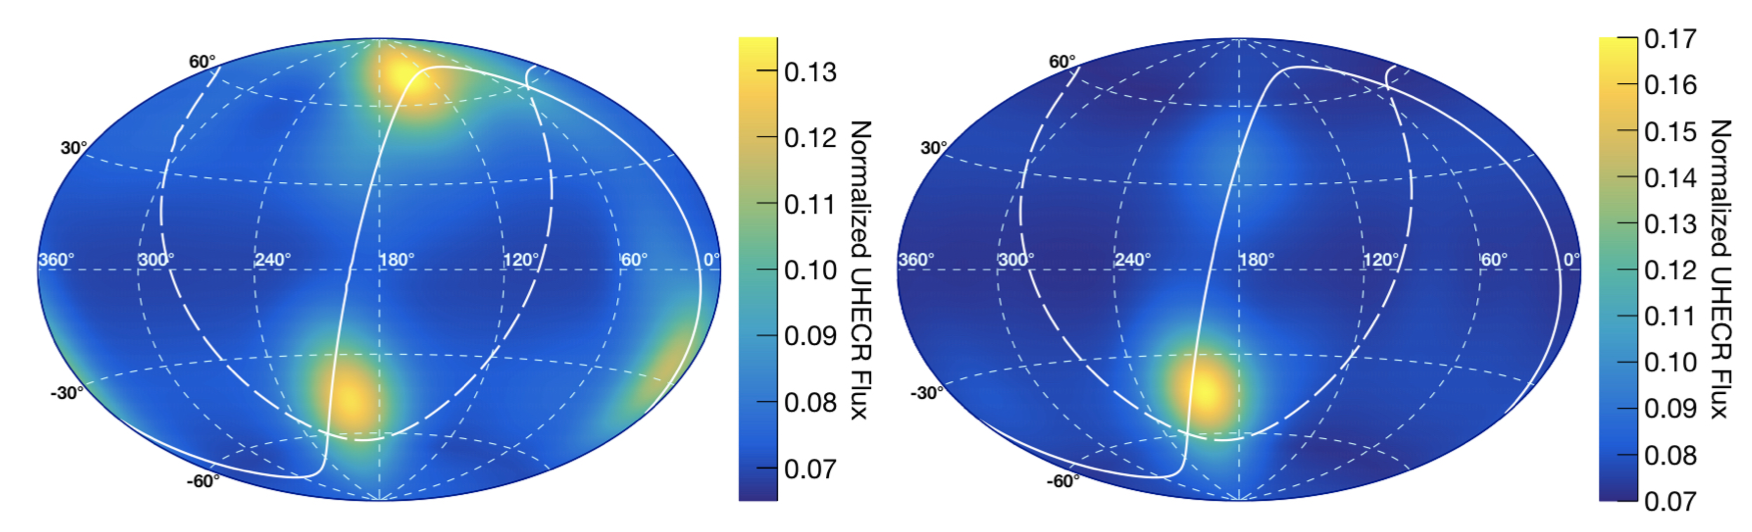
\includegraphics[width=0.65\textwidth]{images/research}    		
	    	
	    	\textit{Sky maps of the normalized UHECR flux. \cite{olintoPOEMMAProbeExtreme2020}} 
    	\end{center}
    	
    \end{block}
\end{column}
\begin{column}{0.55\textwidth - 1cm}


%%%%%%%%%%%%%%%%%%%%%%%%%%%%%%%%%%%%%%%%%%%%%%%%%%%%%
%                 BLOCK: ABSTRACT                   %
%%%%%%%%%%%%%%%%%%%%%%%%%%%%%%%%%%%%%%%%%%%%%%%%%%%%%
    \begin{block}{Talk Abstract}
    	What are the mysterious sources of the most energetic particles ever observed? What astrophysical sources produce very energetic neutrinos? How do particles interact at extreme energies?
		Building on the progress achieved by the ground-based Auger Observatory in studying cosmic particles that reach 100 EeV, an international collaboration is working on space and sub-orbital missions to answer these questions. The Extreme Universe Space Observatory (EUSO) on a super pressure balloon (SPB) is designed to detect ultra-high energy cosmic rays (UHECRs) from above. EUSO-SPB1 flew in 2017 with a fluorescence telescope. EUSO-SPB2 is being built to observe both fluorescence and Cherenkov from UHECRs and neutrinos. These sub-orbital missions lead to POEMMA, the Probe Of Extreme Multi-Messenger Astrophysics, a space mission designed to discover the sources of UHECRs and to observe neutrinos above 20 PeV from energetic transient events. POEMMA will open new Multi-Messenger windows onto the most energetic events in the Universe, enabling the study of new astrophysics and particle physics at these extreme energies.
    \end{block}


%%%%%%%%%%%%%%%%%%%%%%%%%%%%%%%%%%%%%%%%%%%%%%%%%%%%%
%                BLOCK: BACKGROUND                  %
%%%%%%%%%%%%%%%%%%%%%%%%%%%%%%%%%%%%%%%%%%%%%%%%%%%%%
    \begin{block}{Brief Background}
    	The Probe Of Extreme Multi-Messenger Astrophysics (POEMMA) is designed to observe ultra-high-energy cosmic rays (UHECRs) and cosmic neutrinos using space-based measurements of extensive air showers (EASs). POEMMA will monitor colossal volumes of the Earth’s atmosphere to observe the development of EASs produced by UHECRs and UHE neutrinos above 20 EeV and observe the Cherenkov signal from cosmic neutrinos above 20 PeV, in particular from astrophysical transient events.The main scientific goals of POEMMA are to discover the elusive sources of UHECRs and to observe cosmic neutrinos from multi-messenger transients. \cite{olintoPOEMMAProbeExtreme2020}
        \begin{center}
		   	
\includegraphics[width=0.65\textwidth]{images/background}    
		   	
		   		
		   	\textit{Concept of the POEMMA photometer with major components \cite{olintoPOEMMAProbeExtreme2020}}
    	\end{center}
    \end{block}


%%%%%%%%%%%%%%%%%%%%%%%%%%%%%%%%%%%%%%%%%%%%%%%%%%%%%
%                 BLOCK: REFERENCES                 %
%%%%%%%%%%%%%%%%%%%%%%%%%%%%%%%%%%%%%%%%%%%%%%%%%%%%%
    \begin{block}{References}
    	\nocite{*}
        \bibliographystyle{aipnum4-1}
		\bibliography{references}
    \end{block}

\end{column}
\end{columns}


%%%%%%%%%%%%%%%%%%%%%%%%%%%%%%%%%%%%%%%%%%%%%%%%%%%%%
%                    FOOTER TEXT                    %
%%%%%%%%%%%%%%%%%%%%%%%%%%%%%%%%%%%%%%%%%%%%%%%%%%%%%
\begin{textblock}{0.5}(0.18, 0.94)
    \color{white}
    \sffamily
    \textbf{Eberly College of Science}
    \\
    Department of Physics
\end{textblock}


%%%%%%%%%%%%%%%%%%%%%%%%%%%%%%%%%%%%%%%%%%%%%%%%%%%%%
%                   END TEMPLATE                    %
%%%%%%%%%%%%%%%%%%%%%%%%%%%%%%%%%%%%%%%%%%%%%%%%%%%%%
\end{frame}
\end{document}
